


\tikzset{every picture/.style={line width=0.75pt}} %set default line width to 0.75pt        

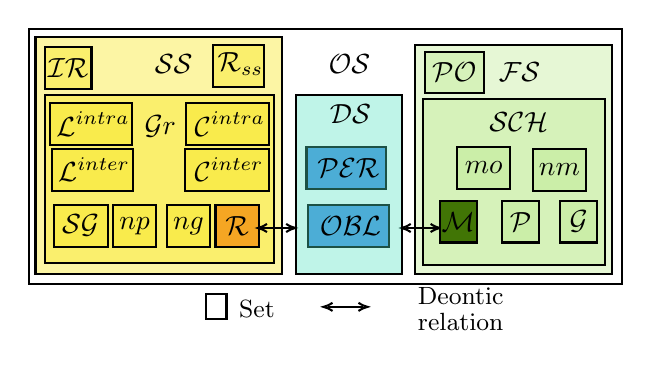
\begin{tikzpicture}[x=0.75pt,y=0.75pt,yscale=-1,xscale=1]
%uncomment if require: \path (0,2639); %set diagram left start at 0, and has height of 2639

%Shape: Rectangle [id:dp6515425466042692] 
\draw  [fill={rgb, 255:red, 255; green, 255; blue, 255 }  ,fill opacity=1 ] (176,834) -- (462,834) -- (462,957) -- (176,957) -- cycle ;
%Shape: Rectangle [id:dp5082212387639646] 
\draw  [fill={rgb, 255:red, 184; green, 233; blue, 134 }  ,fill opacity=0.34 ] (362,842) -- (457.1,842) -- (457.1,952) -- (362,952) -- cycle ;
%Shape: Rectangle [id:dp5297773644830988] 
\draw  [fill={rgb, 255:red, 184; green, 233; blue, 134 }  ,fill opacity=0.34 ] (366,868) -- (453.83,868) -- (453.83,948) -- (366,948) -- cycle ;
%Shape: Rectangle [id:dp1575993513067182] 
\draw  [fill={rgb, 255:red, 248; green, 231; blue, 28 }  ,fill opacity=0.4 ] (179.27,838) -- (298,838) -- (298,952) -- (179.27,952) -- cycle ;
%Straight Lines [id:da8705971767634542] 
\draw    (357.69,930) -- (372,930) ;
\draw [shift={(374,930)}, rotate = 180] [color={rgb, 255:red, 0; green, 0; blue, 0 }  ][line width=0.75]    (4.37,-1.96) .. controls (2.78,-0.92) and (1.32,-0.27) .. (0,0) .. controls (1.32,0.27) and (2.78,0.92) .. (4.37,1.96)   ;
\draw [shift={(355.69,930)}, rotate = 0] [color={rgb, 255:red, 0; green, 0; blue, 0 }  ][line width=0.75]    (4.37,-1.96) .. controls (2.78,-0.92) and (1.32,-0.27) .. (0,0) .. controls (1.32,0.27) and (2.78,0.92) .. (4.37,1.96)   ;
%Shape: Rectangle [id:dp6422856240164194] 
\draw  [fill={rgb, 255:red, 248; green, 231; blue, 28 }  ,fill opacity=0.4 ] (183.81,866) -- (294,866) -- (294,947) -- (183.81,947) -- cycle ;
%Shape: Rectangle [id:dp011814159340156172] 
\draw  [fill={rgb, 255:red, 248; green, 231; blue, 28 }  ,fill opacity=0.4 ] (216.59,919) -- (237.41,919) -- (237.41,939) -- (216.59,939) -- cycle ;

%Shape: Rectangle [id:dp4100462490677821] 
\draw  [fill={rgb, 255:red, 248; green, 231; blue, 28 }  ,fill opacity=0.4 ] (188,919) -- (214,919) -- (214,939) -- (188,939) -- cycle ;
%Shape: Rectangle [id:dp4224844209889693] 
\draw  [fill={rgb, 255:red, 248; green, 231; blue, 28 }  ,fill opacity=0.4 ] (187.02,892) -- (226.03,892) -- (226.03,912) -- (187.02,912) -- cycle ;

%Shape: Rectangle [id:dp2109151755211085] 
\draw  [fill={rgb, 255:red, 248; green, 231; blue, 28 }  ,fill opacity=0.4 ] (186.22,870) -- (225.8,870) -- (225.8,890) -- (186.22,890) -- cycle ;

%Shape: Rectangle [id:dp5612046560441226] 
\draw  [fill={rgb, 255:red, 248; green, 231; blue, 28 }  ,fill opacity=0.4 ] (251.83,870) -- (291.95,870) -- (291.95,890) -- (251.83,890) -- cycle ;

%Shape: Rectangle [id:dp8653779879037786] 
\draw  [fill={rgb, 255:red, 248; green, 231; blue, 28 }  ,fill opacity=0.4 ] (251.29,892) -- (291.72,892) -- (291.72,912) -- (251.29,912) -- cycle ;

%Shape: Rectangle [id:dp5118226471482248] 
\draw  [fill={rgb, 255:red, 65; green, 117; blue, 5 }  ,fill opacity=1 ] (374.01,917) -- (391.99,917) -- (391.99,937) -- (374.01,937) -- cycle ;

%Shape: Rectangle [id:dp9933924068366515] 
\draw  [fill={rgb, 255:red, 248; green, 231; blue, 28 }  ,fill opacity=0.4 ] (242.63,919) -- (263.37,919) -- (263.37,939) -- (242.63,939) -- cycle ;

%Shape: Rectangle [id:dp8500726713846194] 
\draw  [fill={rgb, 255:red, 248; green, 231; blue, 28 }  ,fill opacity=0.4 ] (183.75,843) -- (206.25,843) -- (206.25,863) -- (183.75,863) -- cycle ;

%Shape: Rectangle [id:dp5924732056565294] 
\draw  [fill={rgb, 255:red, 248; green, 231; blue, 28 }  ,fill opacity=0.4 ] (264.98,842) -- (289.16,842) -- (289.16,862) -- (264.98,862) -- cycle ;

%Shape: Rectangle [id:dp346383687870204] 
\draw  [fill={rgb, 255:red, 74; green, 144; blue, 226 }  ,fill opacity=1 ] (309.84,891) -- (348.24,891) -- (348.24,911) -- (309.84,911) -- cycle ;

%Shape: Rectangle [id:dp8336033635496647] 
\draw  [fill={rgb, 255:red, 74; green, 144; blue, 226 }  ,fill opacity=1 ] (310.57,919) -- (349.48,919) -- (349.48,939) -- (310.57,939) -- cycle ;

%Shape: Rectangle [id:dp7738606236066947] 
\draw  [fill={rgb, 255:red, 184; green, 233; blue, 134 }  ,fill opacity=0.34 ] (366.75,845) -- (395.25,845) -- (395.25,865) -- (366.75,865) -- cycle ;

%Shape: Rectangle [id:dp7635846319928088] 
\draw  [fill={rgb, 255:red, 184; green, 233; blue, 134 }  ,fill opacity=0.34 ] (382.43,891) -- (408,891) -- (408,911) -- (382.43,911) -- cycle ;

%Shape: Rectangle [id:dp3026483542328955] 
\draw  [fill={rgb, 255:red, 184; green, 233; blue, 134 }  ,fill opacity=0.34 ] (419.11,892) -- (444.29,892) -- (444.29,912) -- (419.11,912) -- cycle ;

%Shape: Rectangle [id:dp8981167883687693] 
\draw  [fill={rgb, 255:red, 184; green, 233; blue, 134 }  ,fill opacity=0.34 ] (432.02,917) -- (450,917) -- (450,937) -- (432.02,937) -- cycle ;

%Shape: Rectangle [id:dp9543580464730599] 
\draw  [fill={rgb, 255:red, 184; green, 233; blue, 134 }  ,fill opacity=0.34 ] (404,917) -- (421.98,917) -- (421.98,937) -- (404,937) -- cycle ;

%Shape: Rectangle [id:dp9228172603845481] 
\draw  [fill={rgb, 255:red, 245; green, 166; blue, 35 }  ,fill opacity=1 ] (266,919) -- (286.77,919) -- (286.77,939) -- (266,939) -- cycle ;

%Shape: Rectangle [id:dp22226375116176755] 
\draw  [fill={rgb, 255:red, 255; green, 255; blue, 255 }  ,fill opacity=1 ] (261.49,962) -- (271.29,962) -- (271.29,974) -- (261.49,974) -- cycle ;
%Straight Lines [id:da8264214166350665] 
\draw    (320,968) -- (325.86,968) -- (337.25,968) ;
\draw [shift={(339.25,968)}, rotate = 180] [color={rgb, 255:red, 0; green, 0; blue, 0 }  ][line width=0.75]    (4.37,-1.96) .. controls (2.78,-0.92) and (1.32,-0.27) .. (0,0) .. controls (1.32,0.27) and (2.78,0.92) .. (4.37,1.96)   ;
\draw [shift={(318,968)}, rotate = 0] [color={rgb, 255:red, 0; green, 0; blue, 0 }  ][line width=0.75]    (4.37,-1.96) .. controls (2.78,-0.92) and (1.32,-0.27) .. (0,0) .. controls (1.32,0.27) and (2.78,0.92) .. (4.37,1.96)   ;
%Straight Lines [id:da9314770721887407] 
\draw    (302.4,930) -- (288.42,930) ;
\draw [shift={(286.42,930)}, rotate = 360] [color={rgb, 255:red, 0; green, 0; blue, 0 }  ][line width=0.75]    (4.37,-1.96) .. controls (2.78,-0.92) and (1.32,-0.27) .. (0,0) .. controls (1.32,0.27) and (2.78,0.92) .. (4.37,1.96)   ;
\draw [shift={(304.4,930)}, rotate = 180] [color={rgb, 255:red, 0; green, 0; blue, 0 }  ][line width=0.75]    (4.37,-1.96) .. controls (2.78,-0.92) and (1.32,-0.27) .. (0,0) .. controls (1.32,0.27) and (2.78,0.92) .. (4.37,1.96)   ;
%Shape: Rectangle [id:dp058997893239281174] 
\draw  [fill={rgb, 255:red, 80; green, 227; blue, 194 }  ,fill opacity=0.36 ] (304.57,866) -- (356,866) -- (356,952) -- (304.57,952) -- cycle ;


% Text Node
\draw (384.13,969) node  [font=\footnotesize] [align=left] {\begin{minipage}[lt]{59.67pt}\setlength\topsep{0pt}
\begin{center}
{\small Deontic relation}
\end{center}

\end{minipage}};
% Text Node
\draw (286,969) node  [font=\footnotesize] [align=left] {\begin{minipage}[lt]{13.75pt}\setlength\topsep{0pt}
\begin{center}
{\small Set}
\end{center}

\end{minipage}};
% Text Node
\draw (330.5,851) node   [align=left] {$\displaystyle \mathcal{OS}$};
% Text Node
\draw (201,929) node   [align=left] {$\displaystyle \mathcal{SG}$};
% Text Node
\draw (331,875) node   [align=left] {$\displaystyle \mathcal{DS}$};
% Text Node
\draw (245.87,851) node   [align=left] {$\displaystyle \mathcal{SS}$};
% Text Node
\draw (239.38,881) node   [align=left] {$\displaystyle \mathcal{G}r$};
% Text Node
\draw (412.5,855) node   [align=left] {$\displaystyle \mathcal{FS}$};
% Text Node
\draw (412.04,879) node   [align=left] {$\displaystyle \mathcal{SCH}$};
% Text Node
\draw (276.38,929) node   [align=left] {$\displaystyle \mathcal{R}$};
% Text Node
\draw (412.99,927) node   [align=left] {$\displaystyle \mathcal{P}$};
% Text Node
\draw (441.01,927) node   [align=left] {$\displaystyle \mathcal{G}$};
% Text Node
\draw (431.7,902) node   [align=left] {$\displaystyle {nm}$};
% Text Node
\draw (395.21,901) node   [align=left] {$\displaystyle {mo}$};
% Text Node
\draw (381,855) node   [align=left] {$\displaystyle \mathcal{PO}$};
% Text Node
\draw (331,929) node   [align=left] {$\displaystyle \mathcal{OBL}$};
% Text Node
\draw (330,901) node   [align=left] {$\displaystyle \mathcal{PER}$};
% Text Node
\draw (278,851) node   [align=left] {$\displaystyle \mathcal{R}_{ss}$};
% Text Node
\draw (195,853) node   [align=left] {$\displaystyle \mathcal{IR}$};
% Text Node
\draw (253,929) node   [align=left] {$\displaystyle \mathnormal{ng}$};
% Text Node
\draw (383,927) node   [align=left] {$\displaystyle \mathcal{M}$};
% Text Node
\draw (272.51,902) node   [align=left] {$\displaystyle \mathcal{C}^{inter}$};
% Text Node
\draw (272.89,880) node   [align=left] {$\displaystyle \mathcal{C}^{intra}$};
% Text Node
\draw (207,880) node   [align=left] {$\displaystyle \mathcal{L}^{intra}$};
% Text Node
\draw (207.5,902) node   [align=left] {$\displaystyle \mathcal{L}^{inter}$};
% Text Node
\draw (227,929) node   [align=left] {$\displaystyle \mathnormal{np}$};


\end{tikzpicture}